\chapter{Google earth}\label{ap:GE}

Es posible utilizar el \href{https://www.google.com/earth/desktop/}{Google Earth Pro} como herramienta de GIS para analizar los resultados obtenidos(Figura \ref{fig:gearth}). Para ello es necesario exporar la vista como KMZ y luego abrirla en Google Earth.

\begin{figure}[h!]
    \centering
    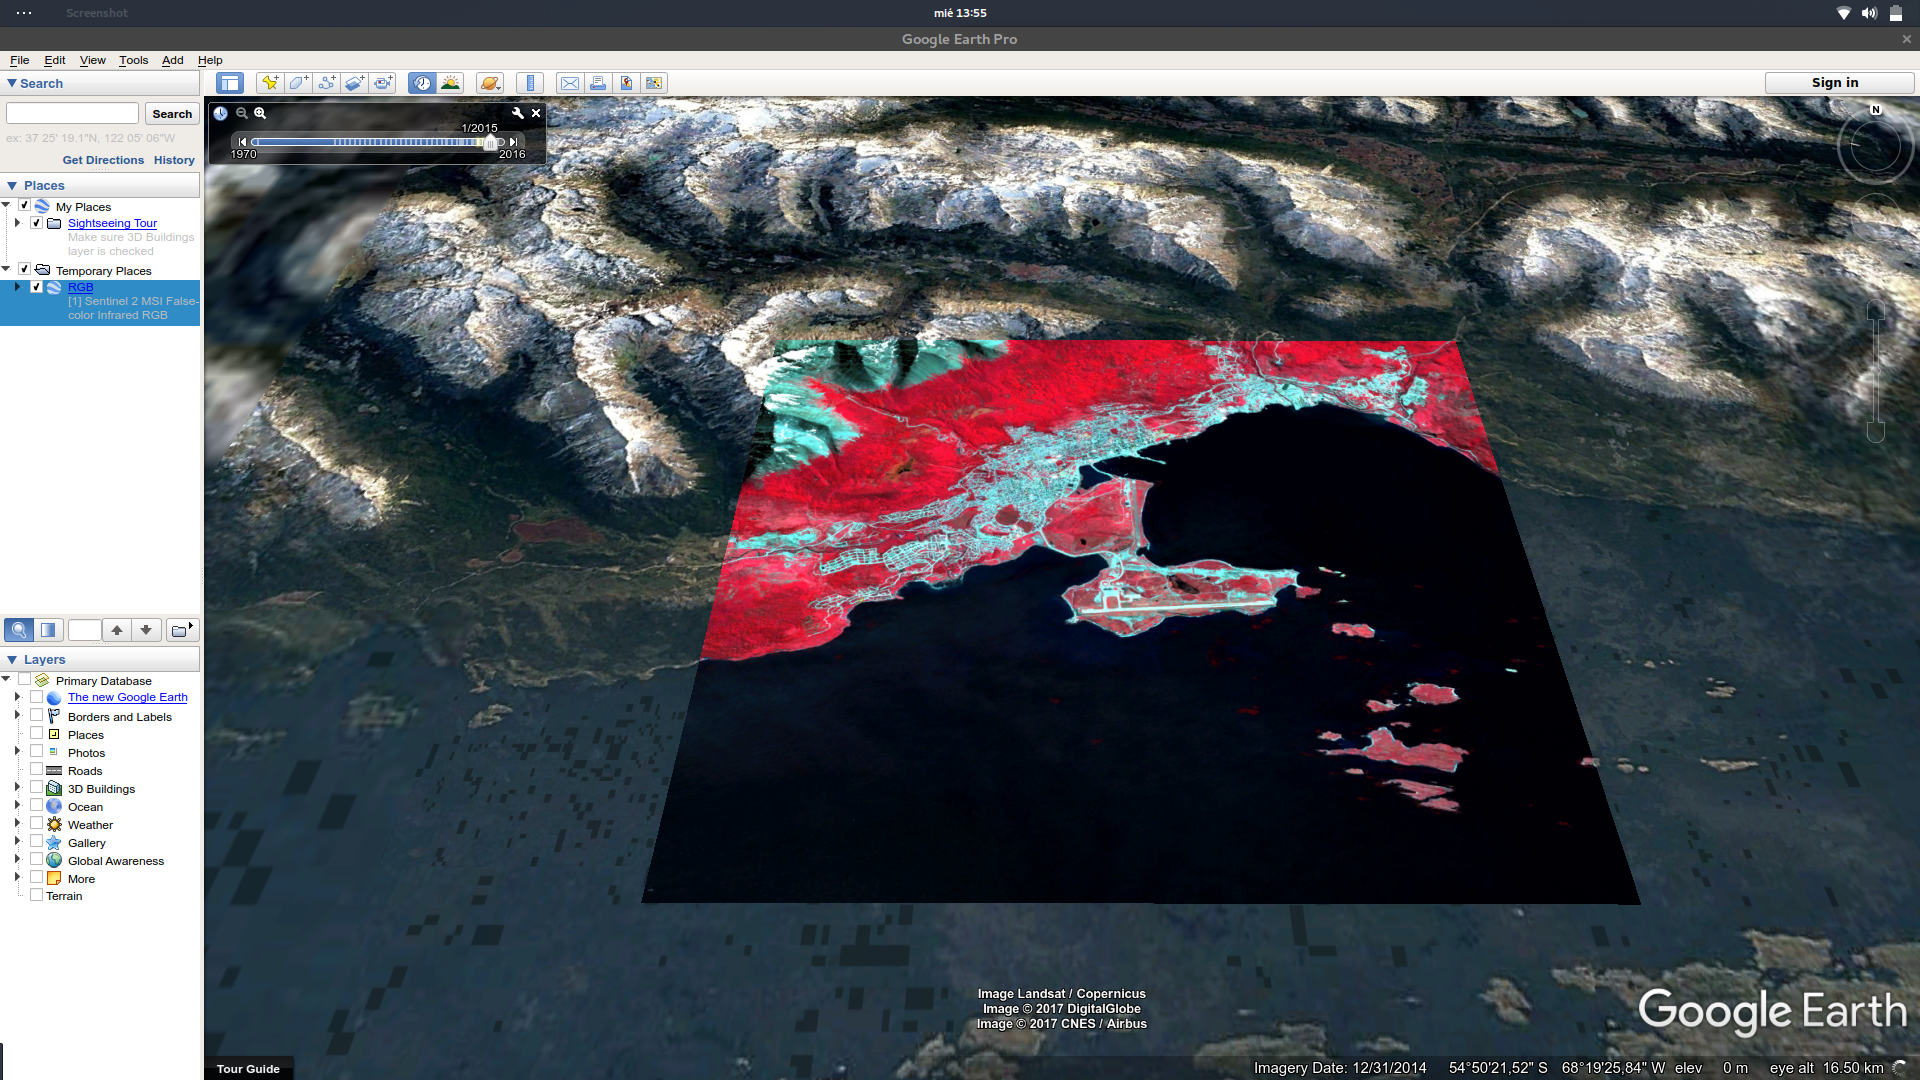
\includegraphics[width=0.7\textwidth]{fig:gearth.png}
    \caption{Imagen óptica de Ushuahia desplegada en Google Earth}
    \label{fig:gearth}
\end{figure}

\section{Creación de archivos KMZ}

Es posible exportar la visualización de la imagen completa o de una región específica desde \menu{File>Export view}. Si selecciona \menu{View as Google Earth KMZ} obtendrá un archivo \texttt{.kmz} que luego podrá abrir desde Google Earth.

Para realizar este proceso la imagen debe encontrarse proyectada en coordenadas geográficas y solo se exportará la vista de la pantalla.

\subsection{Reproyección}

Para reproyectar una imagen vaya al menu \menu{Raster>Geometric>Reprojection}. Aquí deberá seleccionar la imagen de origen como input y la reproyectada como output. Para poder utilizar la imagen deberá elegir en \texttt{Reprojection parameters}, \texttt{Custom CRS} y allí seleccionar \texttt{Projection: Geographi Lat/Lon (WGS 84)} (Figura \ref{fig:reproj}).

\begin{figure}[h!]
    \centering
    \subfloat[I/O Parameters]{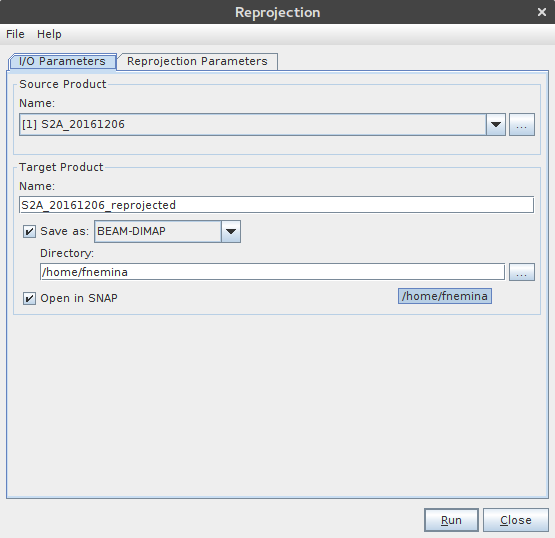
\includegraphics[width=0.35\textwidth]{fig:reproj1.png}}
    \hspace{1cm}
    \subfloat[Processing parameters]{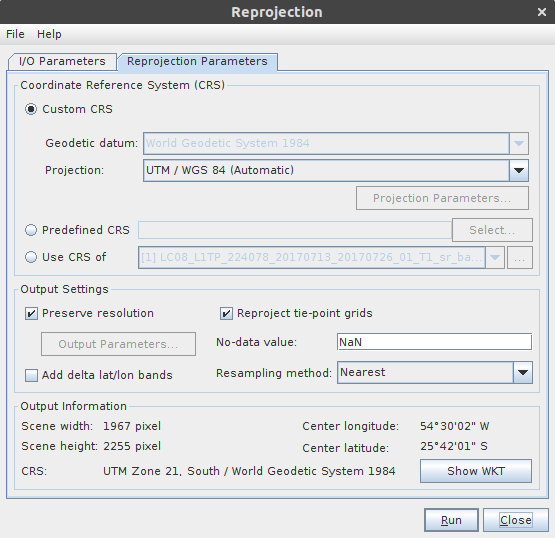
\includegraphics[width=0.35\textwidth]{fig:reproj2.png}}
    \caption{Herramienta de reproyección del SNAP. La imagen se proyecta en coordenadas geográficas.}
    \label{fig:reproj}
\end{figure}

\section{Google earth}

Al ajecutar Google Earth se encontrara con una vista del mundo. Para abrir un archivo \directory{.kmz} dirijasé a \menu{File>Open...}. Seleccione el archivo que exporto del \emph{SNAP} y Google Earth se desplazará automaticamente hasta donde se encuentra el archivo (Figura \ref{fig:gearth}).

Es posible mostrar distintas coberturas seleccionandolas de la sección \menu{Places} a la derecha de la pantalla.
